\documentclass[a4paper,12pt]{article}
\usepackage[top = 2.5cm, bottom = 2.5cm, left = 2.5cm, right = 2.5cm]{geometry}
\usepackage[T1]{fontenc}
\usepackage[utf8]{inputenc}
\usepackage{multirow} 
\usepackage{booktabs} 
\usepackage{graphicx}
\usepackage[spanish]{babel}
\usepackage{setspace}
\setlength{\parindent}{0in}
\usepackage{float}
\usepackage{fancyhdr}
\usepackage{amsmath}
\usepackage{amssymb}
\usepackage{amsthm}
\usepackage[numbers]{natbib}
\newcommand\Mycite[1]{%
	\citeauthor{#1}~[\citeyear{#1}]}
\usepackage{graphicx}
\usepackage{subcaption}
\usepackage{booktabs}
\usepackage{etoolbox}
\usepackage{minibox}
\usepackage{hyperref}
\usepackage{xcolor}
\usepackage[normalem]{ulem}
 \useunder{\uline}{\ul}{}
\usepackage[skins]{tcolorbox}
%---------------------------

\newtcolorbox{cajita}[1][]{
	 #1
}

\newenvironment{sol}
{\renewcommand\qedsymbol{$\square$}\begin{proof}[\textbf{Solución.}]}
	{\end{proof}}

\newenvironment{dem}
{\renewcommand\qedsymbol{$\blacksquare$}\begin{proof}[\textbf{Demostración.}]}
	{\end{proof}}

\newtheorem{problema}{Problema}
\newtheorem{definicion}{Definición}
\newtheorem{ejemplo}{Ejemplo}
\newtheorem{teorema}{Teorema}
\newtheorem{corolario}{Corolario}[teorema]
\newtheorem{lema}[teorema]{Lema}
\newtheorem{prop}{Proposición}
\newtheorem*{nota}{\textbf{NOTA}}
\renewcommand\qedsymbol{$\blacksquare$}
\usepackage{svg}
\usepackage{tikz}
\usepackage[framemethod=default]{mdframed}
\global\mdfdefinestyle{exampledefault}{%
linecolor=lightgray,linewidth=1pt,%
leftmargin=1cm,rightmargin=1cm,
}




\newenvironment{noter}[1]{%
\mdfsetup{%
frametitle={\tikz\node[fill=white,rectangle,inner sep=0pt,outer sep=0pt]{#1};},
frametitleaboveskip=-0.5\ht\strutbox,
frametitlealignment=\raggedright
}%
\begin{mdframed}[style=exampledefault]
}{\end{mdframed}}
\newcommand{\linea}{\noindent\rule{\textwidth}{3pt}}
\newcommand{\linita}{\noindent\rule{\textwidth}{1pt}}

\AtBeginEnvironment{align}{\setcounter{equation}{0}}
\pagestyle{fancy}

\fancyhf{}









%----------------------------------------------------------
\lhead{\footnotesize Geometría Moderna}
\rhead{\footnotesize  Rudik Roberto Rompich}
\cfoot{\footnotesize \thepage}


%--------------------------

\begin{document}
 \thispagestyle{empty} 
    \begin{tabular}{p{15.5cm}}
    \begin{tabbing}
    \textbf{Universidad del Valle de Guatemala} \\
    Departamento de Matemática\\
    Licenciatura en Matemática Aplicada\\\\
   \textbf{Estudiante:} Rudik Roberto Rompich\\
   \textbf{Correo:}  \href{mailto:rom19857@uvg.edu.gt}{rom19857@uvg.edu.gt}\\
   \textbf{Carné:} 19857
    \end{tabbing}
    \begin{center}
        MM2031 - Geometría Moderna - Catedrático: María Eugenia Contreras Pinillos\\
        \today
    \end{center}\\
    \hline
    \\
    \end{tabular} 
    \vspace*{0.3cm} 
    \begin{center} 
    {\Large \bf  HT 1
} 
        \vspace{2mm}
    \end{center}
    \vspace{0.4cm}
%--------------------------

\begin{figure}[H]
	\centering
	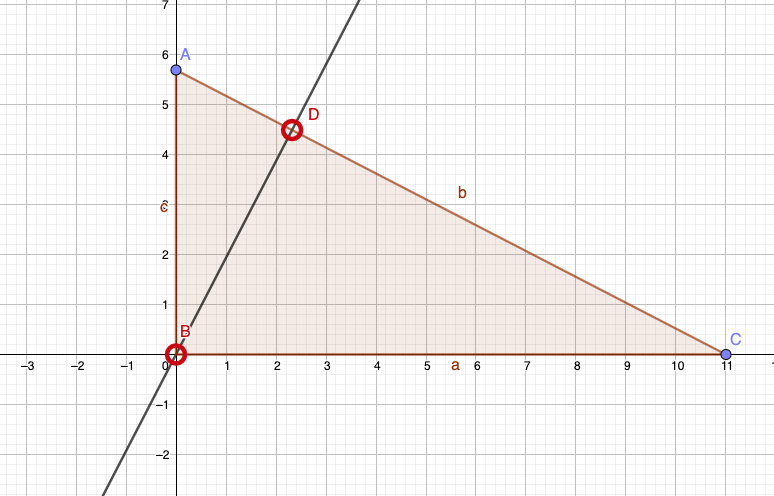
\includegraphics[scale=0.5]{Images/1}
	\caption{Gráficas de los dos problemas}
\end{figure}

\begin{problema}
	La altura sobre la hipotenusa de un triángulo rectángulo divide el triángulo en dos triángulos directamente semejantes, cada uno de los cuales es inversamente semejante al triángulo dado. 
\end{problema}
\begin{dem}
	
	Primer caso: tenemos los triángulos $\triangle ABC$ y $\triangle ABD$. Nótese que $\angle ABC=\angle BDA=90^\circ$. Ahora, tenemos el $\angle DAB=\angle CAB$. Entonces por el criterio $AA$, $\triangle ABC\sim \triangle ABD$. Segundo caso: tenemos los triángulos $\triangle ABC$ y $\triangle DBC$. Nótese que $\angle ABC=\angle CDB=90^\circ$. Ahora, tenemos el $\angle BCA=\angle BCD$. Entonces por el criterio $AA$, $\triangle ABC\sim \triangle  DBC$. Por lo tanto, $\triangle ABC \sim \triangle ABD \sim \triangle DBC$.
\end{dem}

\begin{problema}
	Dado un triángulo rectángulo el producto de longitudes de los catetos es igual al producto de longitudes de la hipotenusa y la altura respectiva.
\end{problema}
\begin{dem}
	A probar: $AB\cdot BC= BD\cdot AC$. Tomando como referencia el problema anterior, 
	$$\frac{BD}{AB}=\frac{DC}{BC}=\frac{BC}{AC}\implies \frac{BD}{AB}=\frac{BC}{AC}\implies AB\cdot BC= BD\cdot AC $$
\end{dem}




%---------------------------
\bibliographystyle{apa}
\bibliography{referencias.bib}

\end{document}